\documentclass[../dissertation.tex]{subfiles}
\begin{document}
Because of the nature of discretisation, there is no absolute guarantee that a curve would not intersect;
this implies that the implementation of the curve untangling process must be carefully designed.
Throughout experiments, common points of failure were:
\begin{itemize}
    \item Some of the edge lengths of the discretised curve became sufficiently large that the quadrature ceased to become valid.
    \item The curves ceased to be smooth (as in Figure \ref{fig: L2 Curve Unknotting} partially).
    \item The curves ``collapsing'' to nullify the kernel, usually after a long time since reaching a stationary state.
        (Figure \ref{fig: Collapse})
    \item Self-intersection in some cases.
\end{itemize}
\begin{figure}[tbp]
    \centering
    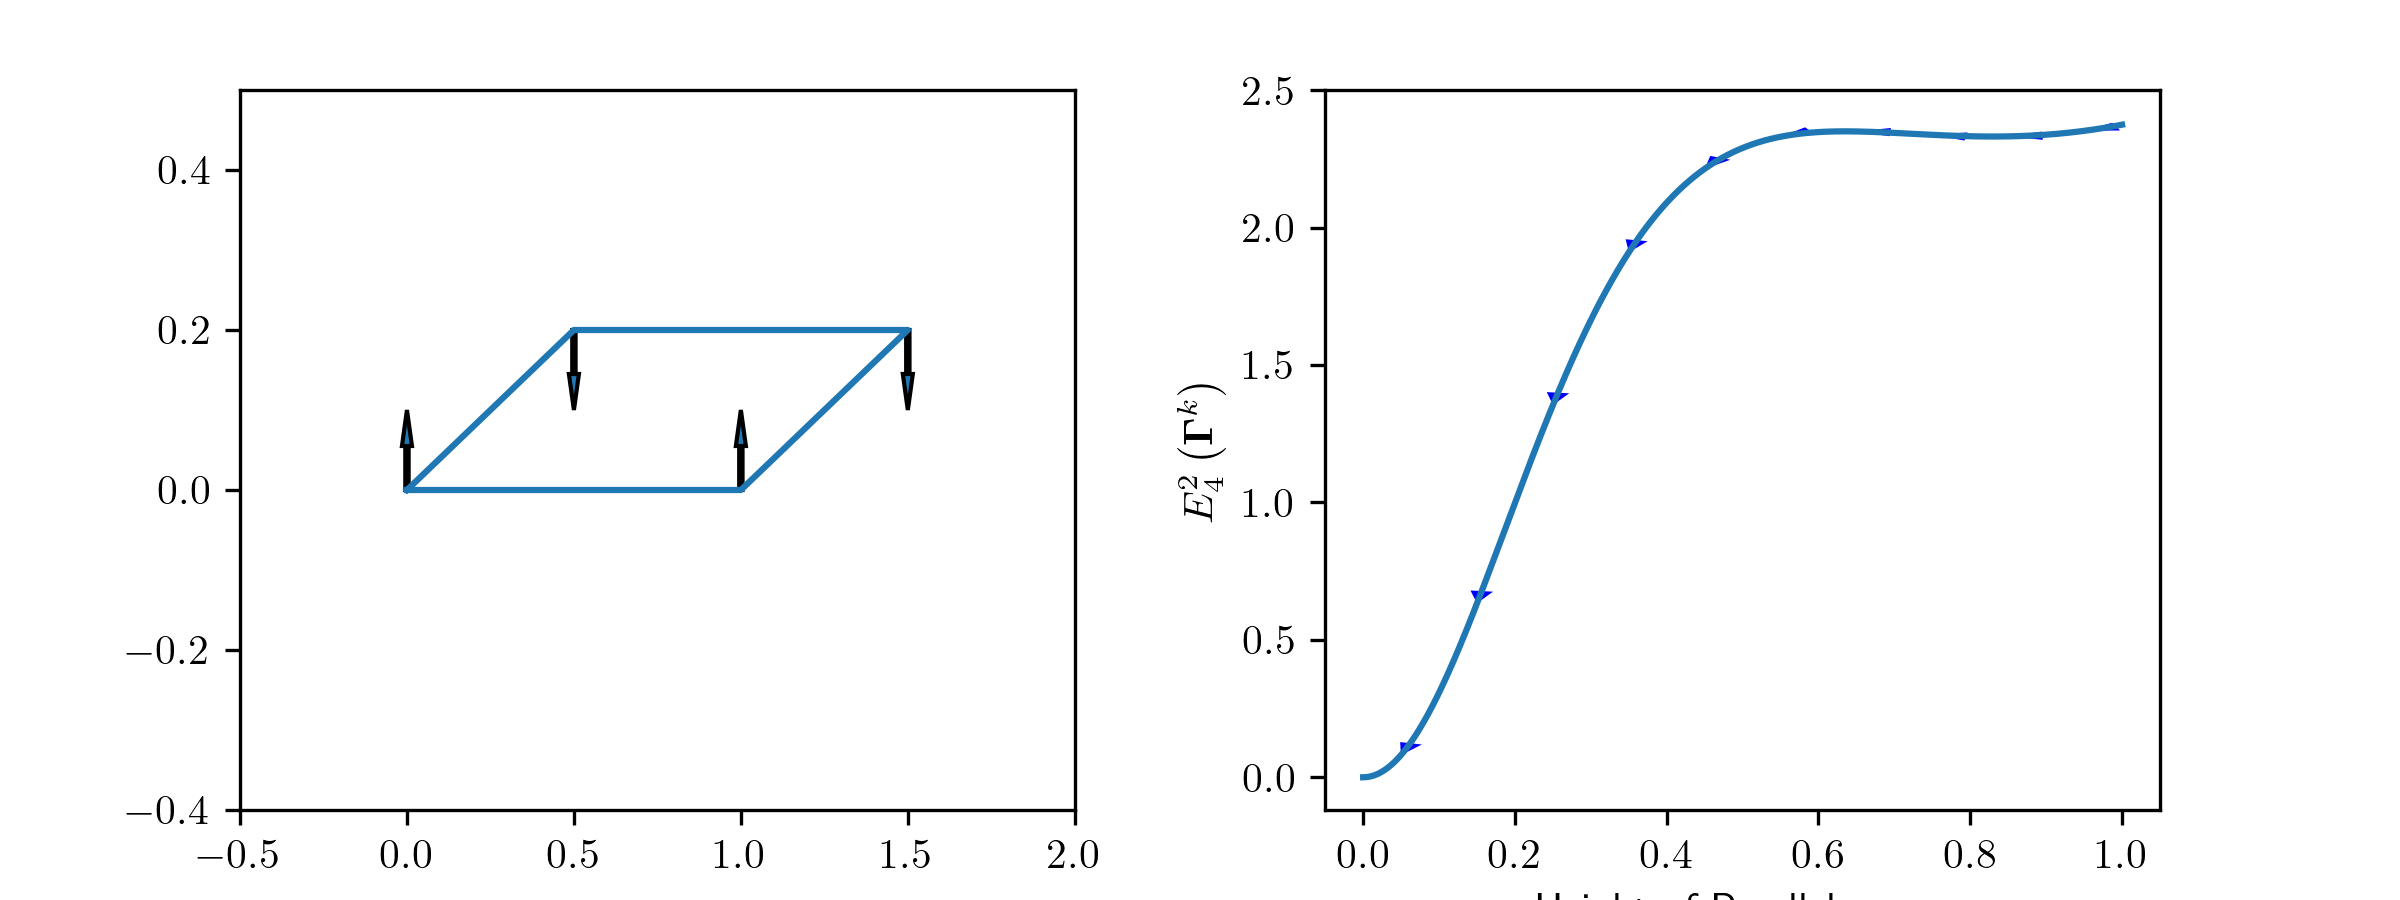
\includegraphics[width=\textwidth]{sections/conclusionImgs/FailureCollapse}
    \caption{
        %For sufficiently low local resolution, the energy can be nullified by a ``collapse'' to a line, as the summand in the quadrature ceases to approximate the actual tangent-point energy kernel.
        In the case of a 4-point discretised curve as shown, while computing the approximate kernel,
        it disregards the adjacent edges, which in fact takes significant portion of the curve out of consideration,
        and does not accurately approximate the kernel of the original curve which the discretised curve came from.
        By taking the height of the parallelogram to zero, all the points align with all the edges $e_i$,
        hence energy is trivially reduced to zero.
    }
    \label{fig: Collapse}
\end{figure}

The simplest idea to resolve some of the arising issues is to take a combination of appropriate constraints as in section \ref{sct: Constraint Energy} to steer the curve away from those issues.
For example, the first point of failure could be fixed by taking the constraint of prescribing edge lengths to be the initial edge lengths. 
Of course, the other points of failure are innate to the approach itself,
and one must tweak the scheme to resolve them.
The nonsmoothness issue can be resolved by using a higher order Sobolev space,
Nullification of the kernel can be resolved by stopping the evolution afer achieving the energy value within a specified tolerance from the energy of the stationary state;
for example, if one attempts evolution of curve which the unknot is a circle, with Buck-Orloff tangent-point energy $\mathcal{E}_{4}^{2}$, we stop the evolution after the energy of the curve is within $\epsilon > 0$ from $\pi^2$,
the Buck-Orloff tangent-point energy of a circle.
For the issue of self-intersection,
it turns out that in practice, taking higher resolution and smaller time step ends up resolving it.

Of course, there are other possible things one could do instead to ameliorate the result of evolution.

\subsection{Possible Variations to Curve Untangling Process}
The most obvious way to improve the evolution is to take smaller time step and higher resolution of the curve.
However, reducing the time step means the evolution itself will be slower,
and increasing resolution means the computation requires more operations per time step,
both of which are undesirable.

\subsubsection{Varying Time Step}
One modification to discrete curve untangling process is to \textbf{vary the time step}.
Instead of using a fixed time step $\Delta T > 0$, one could try modified backtracking Armijo line search\cite{doi:10.1137/1.9781611971200.ch6} as described in Algorithm \ref{alg: Modified bArmijo linesearch}.
(For simplicity, Algorithm \ref{alg: Modified bArmijo linesearch} is expressed for explicit Euler scheme.)
\begin{algorithm}[tbp]
    \caption{Modified backtracking Armijo line search}
    \label{alg: Modified bArmijo linesearch}
    \begin{algorithmic}
        \State Choose constant $0 < \delta < 1$, and $\Delta T^0$ such that after one step of evolution, the curve would not have crossed itself.
        \State Let $k = 0$.
        \State Choose $M > 0$, the number of time steps.
        \While{$k < M$}
        \If{evolution ($\dag$) by time step $\Delta T^k$ requires self-crossing.}
            \State $\Delta T^k \mapsto \delta \Delta T^k$.
            \Else
            \State $\Gammabf^{k+1} \coloneqq \underbrace{\Gammabf^k - \Delta T^k \left( \Grad_X E_{\beta}^{\alpha} \left( \Gammabf^k \right) + \Grad_X C \left( \Gammabf^k \right)\right)}_{(\dag)}$
            \State $k \leftarrow k + 1$
            \EndIf
        \EndWhile
        \Comment{One could choose any other appropriate condition for termination.}
    \end{algorithmic}
\end{algorithm}
Note that time step $\Delta T^k$ decreases only when needed, hence avoids self-crossing;
this gives collision avoidance guarantee\footnote{At least in terms of discretised curve.} by construction\cite{YSC2021}.
However, this requires an algorithm for detecting the change in the isotopy class of the curve.

\subsubsection{Varying the Sample Points}
Another modification of the discrete curve untangling process is to \textbf{vary the sample points}.
When some of the edges of the discrete curve grow disproportionally large compared to most edges,
this can render the tangent-point energy quadrature unusable.
An alternative to adding a constraint energy to fix edge lengths is to resampling points around troublesome edges.
One uses the points around the growing edges to approximate the portion of the curve by a spline. The advantage of this method is that it results in flexibility to change the resolution of the curve sensibly at any time during evolution, at the cost of potential errors which could lead to self-crossing if not careful.

\subsubsection{Discussion of Fractional Sobolev Space}
While this dissertation focused on $L^2$ and $H^1$ gradient flow for the untangling process,
for given $\alpha$ and $\beta$ values for the tangent-point energy,
there is an optimal choice of space for one to implement the curve untangling process,
which makes the evolution by (\ref{equ: Finite Difference Scheme for Curve Untangling Process}) the fastest
and its computation trivial.
It turns out that one could choose the gradient flow over \textbf{fractional Sobolev space} $H^s$
where $s = \frac{\beta - 1}{\alpha}$ to achieve this\cite{YSC2021}.
Just as fractional derivative operators on $\mathbb{R}$ are non-local,
the gradient operator $\grad_{H^s} \mathcal{E}_{\beta}^{\alpha} \left( \Gammabf^k \right)$ over
the generalised Sobolev space $H^s$ is also nonlocal.
This gradient operator relies on the definition of fractional Laplacian\cite{DINEZZA2012521}:
for $s \in \left( 0,1 \right)$,
\begin{align}
    \left( -\laplacian \right)^s u(\xbf) &= C_{n,s} \dashint_{\mathbb{R}^n} \frac{u(\xbf) - u(\ybf)}{\norm{\xbf - \ybf}^{n+2s}} \intd V_{\ybf} \\
    &= -\frac{1}{2} C_{n,s} \int_{\mathbb{R}^n} \frac{u\left( \xbf + \ybf \right) + u\left( \xbf - \ybf \right) - 2 u(\xbf)}{\norm{\ybf}^{n+2s}} \intd V_{\ybf} \\
    &= \mathcal{F}^{-1} \left( \norm{\xibf}^{2s} \left( \mathcal{F} u \right) \right)
\end{align}
where $\mathcal{F}$ is the Fourier transform operator, $\dashint$ is the principal value integral as in the definition of inverse Fourier transform, and $C_{n,s}$ is some constant that makes the last equality valid.
It is sensible to attempt nonlocal gradient operator in the gradient flow, as the tangent-point energy itself is, in some sense, nonlocal.

\end{document}
